%================================================================
% 作業ログ 2026-06-23（回路実作成・マイコン破損・リポジトリ公開化）
%   ユニバーサル基板に MPU-9250 + ESP32-S3 を手はんだ実装，
%   配線ミスでマイコンを破損し代替品を発注．
%   リポジトリをパブリックに変更．ソフトウェア開発の進捗なし．
%
%   ビルド:
%     cd work/shiozawa/work-0623/作業ログ0623
%     docker run --rm -v "$(pwd):/workspace" -w /workspace \
%       ghcr.io/paperist/texlive-ja:debian latexmk 作業ログ0623.tex
%================================================================
\documentclass[uplatex,dvipdfmx,a4paper,11pt]{jsarticle}

% --- 余白 ---
\usepackage[top=25mm,bottom=25mm,left=25mm,right=25mm]{geometry}

% --- 表・箇条書き・図・色 ---
\usepackage{array}
\usepackage{tabularx}
\usepackage{booktabs}
\usepackage{enumitem}
\usepackage{graphicx}
\usepackage{url}
\usepackage[table]{xcolor}
\usepackage{amssymb}

% --- 段落間隔（Wordのような見た目に寄せる）---
\setlength{\parindent}{0pt}
\setlength{\parskip}{0.6em}

% --- セクション見出しを「番号. 太字」+ 章末に水平線を入れる ---
\usepackage{titlesec}
\titleformat{\section}
  {\normalfont\Large\bfseries}{\thesection.}{0.6em}{}
\titleformat{\subsection}
  {\normalfont\large\bfseries}{\thesubsection}{0.6em}{}
\titlespacing*{\section}{0pt}{1.2em}{0.6em}
\titlespacing*{\subsection}{0pt}{1.0em}{0.4em}

% --- 章末水平線（手で \sectionrule と書いて区切る）---
\newcommand{\sectionrule}{\par\medskip\noindent\rule{\linewidth}{0.6pt}\par\medskip}

% --- 箇条書きの記号を Word 風（・→○→数字）に揃える ---
\renewcommand{\labelitemi}{\textbullet}
\renewcommand{\labelitemii}{\textopenbullet}
\setlist[itemize]{leftmargin=1.6em,itemsep=0.1em,topsep=0.2em}
\setlist[enumerate]{leftmargin=2.0em,itemsep=0.1em,topsep=0.2em}

% \textopenbullet が無い環境向けのフォールバック
\providecommand{\textopenbullet}{\ensuremath{\circ}}

% --- 進捗ガントチャート用（グリッド表）---
\definecolor{barDone}{gray}{0.55} % 完了
\definecolor{barProg}{gray}{0.78} % 進行中
\definecolor{barPlan}{gray}{0.90} % 予定
\definecolor{nowCol}{gray}{0.30}  % 今週の見出し
\newcolumntype{G}{>{\centering\arraybackslash}p{2.0em}}
\newcommand{\bD}{\cellcolor{barDone}}
\newcommand{\bP}{\cellcolor{barProg}}
\newcommand{\bQ}{\cellcolor{barPlan}}

\begin{document}

%================================================================
% ヘッダ
%================================================================
{\LARGE\bfseries 作業ログ}\par\bigskip

報告者：塩澤 匠生

報告日：2026年6月23日

プロジェクト名：タクトーン~ IMUジェスチャーで奏でるArduinoオーケストラ~ \\

\sectionrule

%================================================================
% 1. 進捗サマリー
%================================================================
\section{進捗サマリー（要約）}

\begin{itemize}
  \item 全体進捗率：70\%（先週から変化なし．回路の実作成に時間を費やしたが配線ミスで
        マイコンを破損し，代替品を発注した．ソフトウェア開発の進捗はなし）
  \item 進捗状況（今週の変化）：
    \begin{itemize}
      \item ユニバーサル基板に MPU-9250 IMU センサーモジュール + ESP32-S3-N16R8 開発ボードを手はんだで実装（約 1 時間半）
      \item 配線ミスによりマイコン（ESP32-S3-N16R8）を破損
      \item 壊したマイコンの代替品を発注
      \item リポジトリをパブリックに変更し，先生方がリポジトリを閲覧できるようにした
    \end{itemize}
  \item 今週の主要成果：
    \begin{itemize}
      \item 回路の実物が形になった（図\ref{fig:board-front}，図\ref{fig:board-back}参照）
      \item リポジトリの公開化により，先生方への成果物共有が容易になった
    \end{itemize}
  \item 重大課題（影響度：高）：
    \begin{itemize}
      \item {}[配線ミスでマイコンを破損．代替品の到着まで実機テストが停止する．
            発表会（7/1）までの残り日数が少なく，到着後は迅速にテストを再開する必要がある]
    \end{itemize}
\end{itemize}

\sectionrule

%================================================================
% 2. 進捗ガントチャート（計画と現在地）
%================================================================
\section{進捗ガントチャート（計画と現在地）}

チームのガントチャート（\texttt{meetings/ガントチャーver1ト.xlsx}）のフェーズ区分（110 基本設計／
120 詳細設計／200 実装／300 テスト／400 ストレッチ）に，現在の進み具合を重ねたもの．
「今」の縦位置は本報告時点（6 月第 4 週）．

\medskip
{\footnotesize
\setlength{\tabcolsep}{2pt}
\renewcommand{\arraystretch}{1.2}
\begin{tabular}{@{}p{8.5em}|*{12}{G}@{}}
 & & & & & & & & & & & \multicolumn{1}{c}{$\downarrow$今} & \\
作業項目（フェーズ）
 & \cellcolor{barPlan}\tiny 4/15 & \cellcolor{barPlan}\tiny 4/22 & \cellcolor{barPlan}\tiny 4/29
 & \cellcolor{barPlan}\tiny 5/6 & \cellcolor{barPlan}\tiny 5/13 & \cellcolor{barPlan}\tiny 5/20
 & \cellcolor{barPlan}\tiny 5/27 & \cellcolor{barPlan}\tiny 6/3 & \cellcolor{barPlan}\tiny 6/10
 & \cellcolor{barPlan}\tiny 6/17 & \cellcolor{nowCol}\tiny\textcolor{white}{6/24} & \cellcolor{barPlan}\tiny 7/1 \\
\midrule
企画・テーマ決定        & \bD & \bD &     &     &     &     &     &     &     &     &     &     \\
110 基本設計            &     &     & \bD & \bD &     &     &     &     &     &     &     &     \\
120 詳細設計            &     &     &     &     & \bD &     &     &     &     &     &     &     \\
\textbf{200 実装}       &     &     &     &     &     &     &     &     &     &     &     &     \\
\quad test\_v2 輪唱・同期 &     &     &     & \bD & \bD & \bD & \bD &     &     &     &     &     \\
\quad test\_v3 ゲーム(firmware) &  &     &     &     &     & \bD & \bD & \bD & \bD &     &     &     \\
\quad test\_v3 Processing &   &     &     &     &     &     & \bD & \bD & \bD &     &     &     \\
\textbf{300 テスト}     &     &     &     &     &     &     &     &     &     &     &     &     \\
\quad 単体・結合・システム &   &     &     &     &     &     &     &     & \bP & \bP & \bP &     \\
\quad 評価（精度・遅延） &     &     &     &     &     &     &     &     &     &     & \bQ & \bQ \\
400 ストレッチ（強弱ほか） &  &     &     &     &     &     &     & \bQ & \bQ &     &     &     \\
発表会                  &     &     &     &     &     &     &     &     &     &     &     & \multicolumn{1}{c}{$\bigstar$} \\
\bottomrule
\end{tabular}
}

\medskip
凡例：\colorbox{barDone}{~~}~完了 \quad \colorbox{barProg}{~~}~進行中 \quad
\colorbox{barPlan}{~~}~予定 \quad $\bigstar$~発表会（7/1）

\medskip
※ 今週は回路の手はんだ作業に注力したが配線ミスでマイコンを破損し，代替品到着待ち．
テストフェーズは机上検証（前週完了）以降，実機テストが停滞している．

\sectionrule

%================================================================
% 3. 作業ログ（詳細トラッキング）
%================================================================
\section{作業ログ（詳細トラッキング）}

\begin{tabularx}{\linewidth}{@{}p{10em}p{6em}p{4em}p{3em}X@{}}
\toprule
作業項目 & 実施日 & 作業時間 & 進捗 & コメント \\
\midrule
回路の手はんだ実装 & 2026-06-23 & 90 分 & 80\% & ユニバーサル基板に MPU-9250 IMU センサーモジュール + ESP32-S3-N16R8 開発ボードを手はんだで配線．配線ミスによりマイコンを破損 \\
マイコンの発注 & 2026-06-23 & 10 分 & 100\% & 破損した ESP32-S3-N16R8 の代替品を発注 \\
リポジトリ公開化 & 2026-06-23 & 5 分 & 100\% & GitHub リポジトリをプライベートからパブリックに変更．先生方が閲覧可能に \\
\midrule
\multicolumn{2}{@{}l}{\textbf{合計}} & \textbf{105 分} & & \\
\bottomrule
\end{tabularx}

\sectionrule

%================================================================
% 4. 課題管理
%================================================================
\section{課題管理}

\begin{tabularx}{\linewidth}{@{}p{8em}Xp{2.5em}p{2.5em}Xp{3em}@{}}
\toprule
課題 & 発生原因 & 影響度 & 優先度 & 対策 & 状態 \\
\midrule
マイコン破損 & 手はんだ時の配線ミス & 高 & 高 & 代替品を発注済み．到着後に正しい配線で再実装する & 対応中 \\
実機で輪唱が聞こえない & 楽器ファームの書き込み取り違えが有力仮説（前週からの継続） & 高 & 高 & マイコン到着後に test\_v3 main を全楽器に書き込み直して切り分け & 継続 \\
SW 進捗の停滞 & 回路作業に時間を取られた & 中 & 高 & マイコン到着待ちの間に SW 側の作業（テスト準備・発表資料）を進める & 対応中 \\
UDP マルチキャストのパケロス & ACK・再送なし & 中 & 中 & 連送 4 発＋WiFi 復帰時再 join で対策済み．実機テストで効果確認する & 継続 \\
\bottomrule
\end{tabularx}

\medskip
※影響度＝プロジェクトへのインパクト，優先度＝対応の緊急性

\sectionrule

%================================================================
% 5. AI利用状況と検証
%================================================================
\section{AI利用状況と検証(再現性重視)}

\subsection{利用内容}

\begin{itemize}
  \item 今週はハードウェア（手はんだ）作業が中心であり，AI の利用はなし
\end{itemize}

\sectionrule

%================================================================
% 6. 次回計画
%================================================================
\section{次回計画}

\begin{itemize}
  \item 目標：
    \begin{itemize}
      \item {}[代替マイコン到着後，正しい配線で回路を再実装する]
      \item {}[test\_v3 main を全楽器に書き込み直し，輪唱の実機確認を行う]
      \item {}[発表会（7/1）に向けた準備（発表資料・デモ構成）を開始する]
    \end{itemize}
  \item 達成基準：
    \begin{itemize}
      \item {}[回路が正常に動作し，IMU データを取得できる状態になる]
      \item {}[発表会のデモ構成が決まっている]
    \end{itemize}
  \item 期限：
    \begin{itemize}
      \item {}[7/1 発表会までにデモ可能な状態に持っていく]
    \end{itemize}
\end{itemize}

\sectionrule

%================================================================
% 7. その他
%================================================================
\section{その他}

\begin{itemize}
  \item {}[回路の手はんだ作業自体は形になったが（図\ref{fig:board-front}，
        図\ref{fig:board-back}），配線ミスでマイコンを破損してしまった．
        代替品の到着を待って再実装する]
  \item {}[リポジトリをパブリック化したことで，先生方に GitHub 上で直接
        ソースコードや進捗を確認していただける状態になった]
  \item {}[発表会まで残り 1 週間．マイコン到着までの間はソフトウェア側の
        作業（テスト準備・発表資料）を並行して進める必要がある]
\end{itemize}

\sectionrule

%================================================================
% 8. 付録
%================================================================
\section{付録}

\begin{itemize}
  \item 添付資料：
    \begin{itemize}
      \item 回路写真：図\ref{fig:board-front}（表面），図\ref{fig:board-back}（裏面）
      \item GitHub リポジトリ：\url{https://github.com/takushio2525/2026-hackathon-team23}
    \end{itemize}
  \item 添付範囲：
    \begin{itemize}
      \item 今週の作業成果物（回路基板の写真 2 枚）
    \end{itemize}
\end{itemize}

\bigskip

% --- 回路写真 ---
\begin{figure}[h]
  \centering
  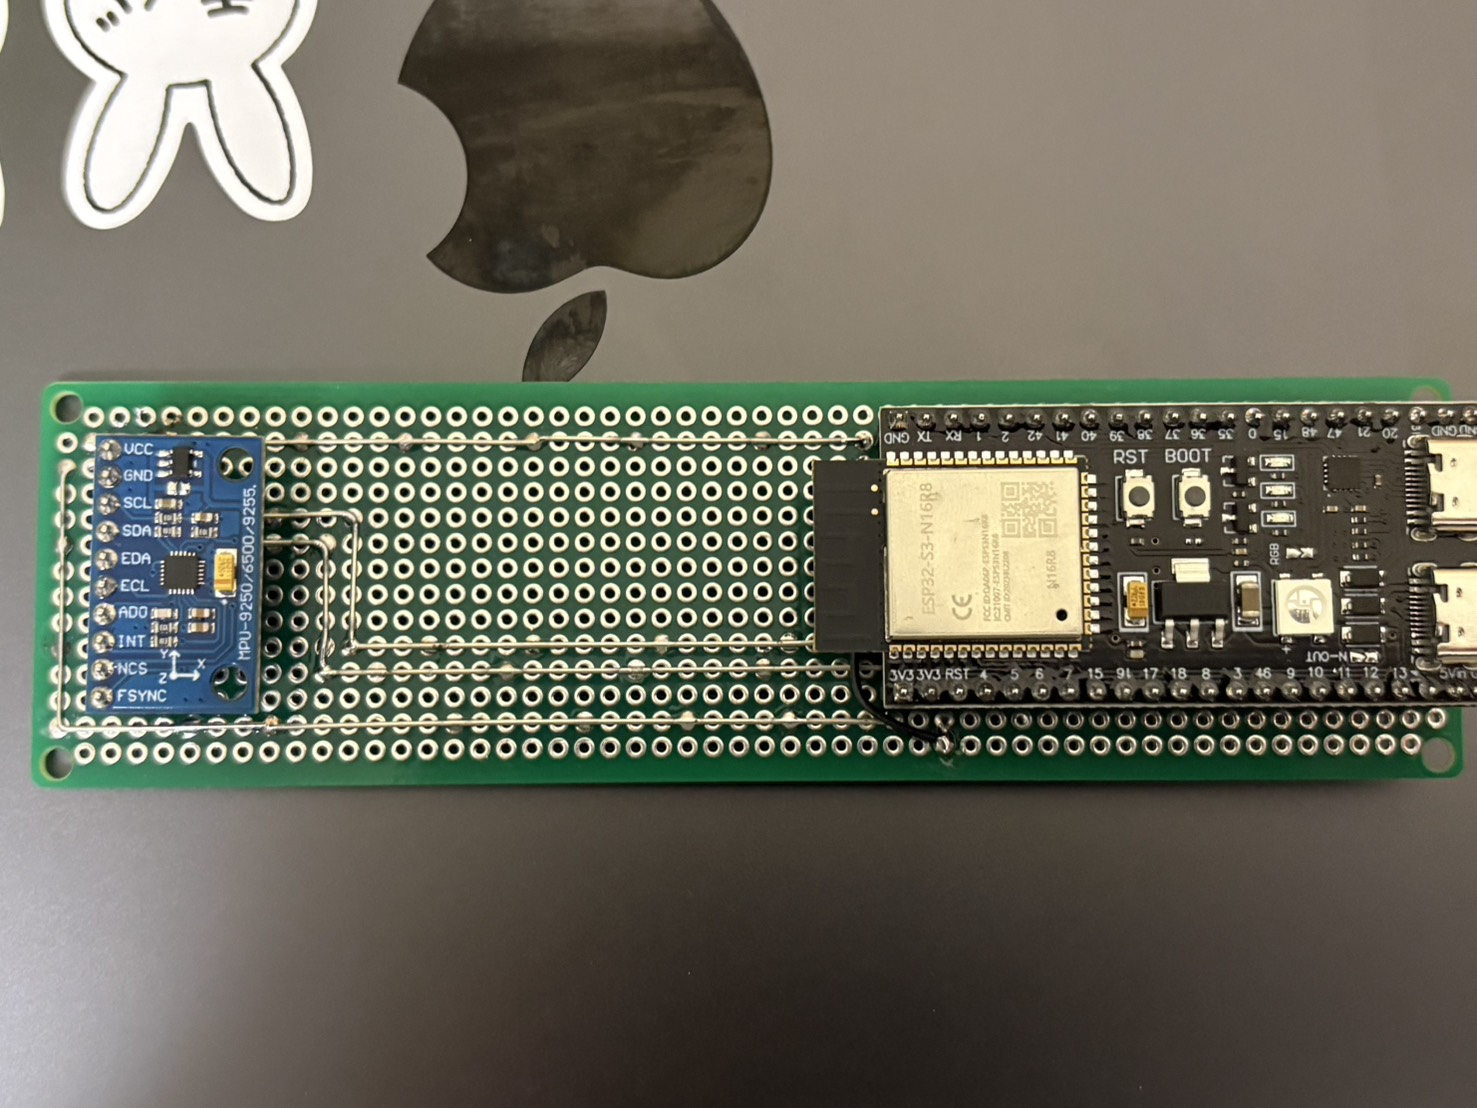
\includegraphics[width=0.7\linewidth]{fig/board_front.png}
  \caption{指揮者ノード基板（表面）：ユニバーサル基板に MPU-9250 IMU センサーモジュール（左）と
    ESP32-S3-N16R8 開発ボード（右）を手はんだで実装}
  \label{fig:board-front}
\end{figure}

\begin{figure}[h]
  \centering
  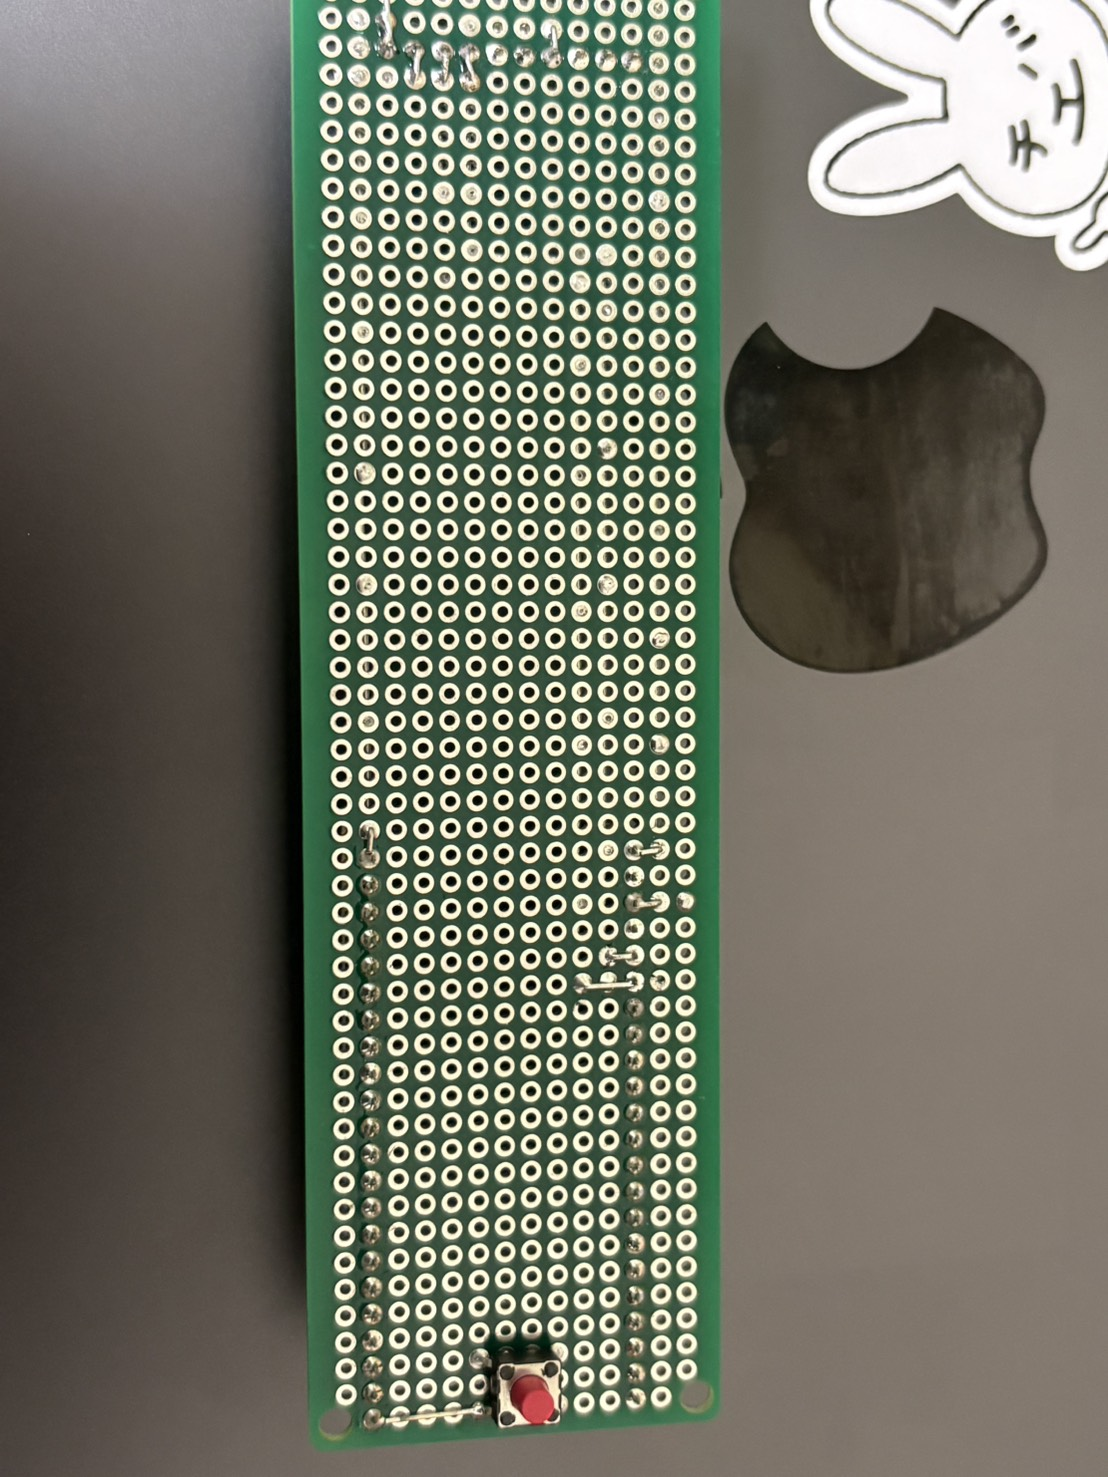
\includegraphics[width=0.5\linewidth]{fig/board_back.png}
  \caption{指揮者ノード基板（裏面）：はんだ配線の跡．下部にタクトスイッチ}
  \label{fig:board-back}
\end{figure}

\sectionrule

\end{document}
